\label{KostenundArbeitsplan}

Die Kosten des Projektes belaufen sich, wie in \ref{tab:Kosten} nachzuvollziehen ist, auf 73,14€. An dieser Stelle muss jedoch angefügt werden, dass es sich hierbei nicht um die reinen Materialkosten für das Projekt handelt, da beispielsweise das Arduinoset einiges mehr, als nur die benötigten Materialien bietet. Somit kann man sagen, dass sich die Kosten bei einer Bestellung mit Einschränkung auf die benötigten Komponenten senken würden.

\begin{table}[!hbt]
	
	\centering
	
	\begin{tabular}{|p{8cm}|p{8cm}|}
		
		\hline
		\rowcolor{lightgray} Einkauf & Kosten \\
		\hline
		Arduinoset & 27,95€ \\
		\hline
		CO2-Sensor (CCS811) & 8,50€ \\
		\hline
		MikroSD-Modul & 3,50€ \\
		\hline
		LED-Fassung & 4,59€ \\
		\hline
		Mechanische Bauteile & 24,99€ \\
		\hline
		Sonstiges & 4,56€ \\
		\hline
		\rowcolor{lightgray} Gesamt & 73,14€ \\
		\hline
		
	\end{tabular}
	
	\captionabove{Aufgewendete Kosten für das Projekt}
	\label{tab:Kosten}
	
\end{table}

Damit wir zu jedem Zeitpunkt einschätzen können, ob wir im Zeitplan sind, haben wir zu Beginn des Jahres den in Abbildung \ref{fig:Ablaufplan} zu sehenden Projektplan erstellt. An diesen Ablauf inklusive den Daten, hat sich jedes Gruppenmitglied zu halten. Eine Verzögerung in der Entwicklung, bedeutet eine Verschiebung der Abwicklung des Projektes. Davon hängt somit die Fertigstellung, als auch der Erfolg des Projektes ab.

\begin{figure}[!hbt]
	\centering
	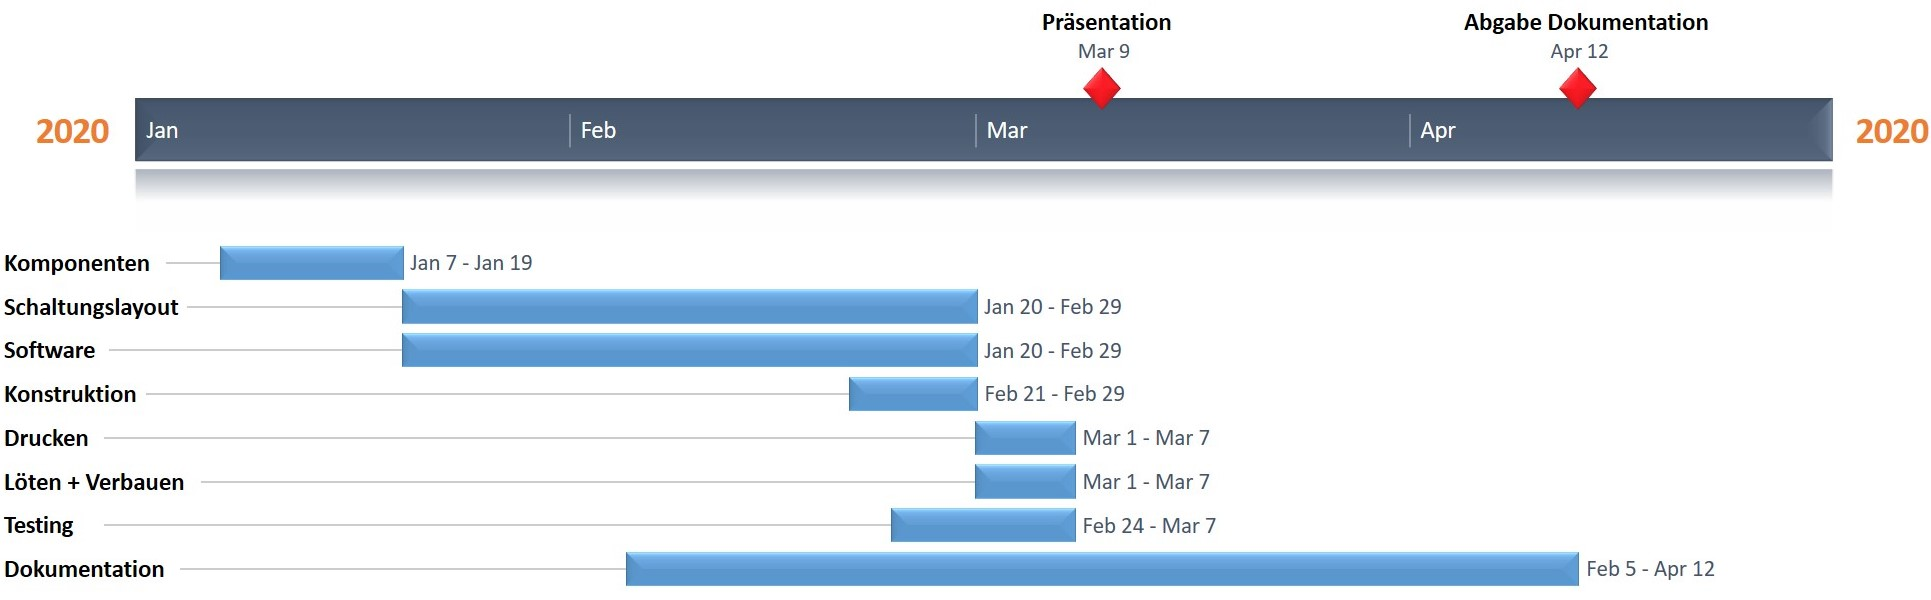
\includegraphics[width=1\linewidth]{Images/Ablaufplan}
	\caption{Ablauf des Projektes von Januar bis April}
	\label{fig:Ablaufplan}
\end{figure}

Auch, wenn die Abgabefrist erst vier Wochen nach Semesterende abläuft, haben wir uns, wie in Abbildung \ref{fig:Ablaufplan} zu sehen ist, den 12. April als Meilenstein für die Abgabe des Projektes gesetzt. Die Begründung für diese Entscheidung liegt zum einen darin, dass wir bei Problemen bezüglich der Abgabe einen gewissen Puffer haben. Zum anderen beginnt ab Anfang April die dritte Praxisphase der dualen Studierenden, in welcher sie ab Mitte des Monats schon in ihrem neuen Projekt vertieft sind und somit weniger Zeit für das Mikrocomputertechnik-Projekt aufwenden können.